\section{问题二的建模与求解}

\subsection{问题分析框架}

设正向映射算子 $F$ 将纸面图案映射为镜面图案：$I_M = F(I_P)$。问题二分两个层次：层次1（自由设计）要求纸面图案 $I_P$ 和 $F(I_P)$ 均有语义；层次2（指定镜面）给定目标镜面图案 $I_M^*$，要求纸面图案 $I_P = f^{-1}(I_M^*)$ 经艺术加工后也有语义。两个层次的核心挑战均在于：圆柱反射映射会对纸面图案施加非线性几何变换，如何在变换前后同时保持视觉语义的可辨识性。

\subsection{层次1：自由设计的可行性分析}

圆柱反射的几何特性是\textbf{环向拉伸+径向压缩}：靠近圆柱的纸面区域，$\theta$ 方向（环向）被拉伸，$h$ 方向（径向）被压缩。若纸面图案具有 $n$ 重旋转对称性（如 $n=4$ 的十字形、$n=6$ 的雪花形），则正向映射后的镜面图案在环向方向上呈现周期性重复结构，天然具有视觉规律性。

\textbf{频谱分离原理}是层次1可行性的理论基础\cite{mallat_wavelet_2009,gonzalez_digital_2018}。设纸面图案的频谱为 $\hat{I}_P = \hat{I}_P^{\text{low}} + \hat{I}_P^{\text{high}}$，其中低频分量（空间频率 $< f_c$）决定图案的整体视觉语义，高频分量决定反射细节。由于圆柱反射映射的低通特性（雅可比行列式的平滑性），高频纸面信息在镜面图案中被衰减，而低频信息被保留。这意味着可以在纸面图案中叠加低频语义信息（如大尺度轮廓），而不显著影响镜面图案的质量。因此，层次1的可行性较高，尤其是放射状、旋转对称等与圆柱反射机制天然适配的图案。

\subsection{层次2：指定镜面图案后的纸面语义保持}

逆映射将圆柱展开面（矩形）映射到纸面（扇形区域），产生以下视觉效果：环向方向（$\theta$ 变化）映射到纸面上的弧形曲线，产生弯曲效果；径向方向（$h$ 变化）映射到纸面上的放射状线条，产生发散效果。因此，逆映射后的纸面图案天然具有\textbf{放射状/扇形}的视觉结构，与太阳/光芒图案、花朵/曼陀罗图案、抽象装饰纹样等有意义图案兼容。

艺术加工策略包括四个方面：（1）色彩重映射，将纸面图案的灰度值映射到艺术色彩方案；（2）背景填充，在圆柱投影区域外填充有意义的背景图案；（3）轮廓强化，沿纸面图案的主要轮廓线添加装饰性描边；（4）对称补全，利用圆柱反射的对称性将纸面图案扩展为完整的对称图案。这四种策略可以单独使用，也可以组合叠加，灵活适应不同的设计需求。

\subsection{具体案例构造与验证}

为验证上述理论分析的可行性，本文构造了3个具体案例，通过逆映射生成纸面图案后叠加艺术化背景，并用SSIM验证镜面图案的可辨识度。三个案例覆盖了从简单几何到复杂对称图案的不同难度层次，具有代表性。

\subsubsection{案例1：文字镜面图案与放射状纸面图案}

案例1以文字"ART"为目标镜面图案，探索最简单的低频语义图案的可行性。圆柱参数取 $R=15$ mm，$H=50$ mm，$\phi=\pi$，$\alpha=60°$。目标镜面图案为黑底白字"ART"，字体采用粗体无衬线字体，笔画宽度约为图案高度的15\%，确保在几何变换后仍可辨识。

通过逆映射生成纸面图案后，纸面图案呈现放射状弯曲线条，这是文字笔画经圆柱反射逆变换后的自然结果。艺术加工将线条着色为金色渐变（从中心向外由深金色过渡到浅金色），背景填充深蓝色，整体呈现为装饰性放射花纹，具有明显的视觉美感。案例1的纸面图案与镜面仿真效果如图\ref{fig:case1}所示。

\begin{figure}[H]
\centering
\subfloat[目标镜面图案（文字"ART"）]{
\includegraphics[width=0.30\textwidth]{../figures/case1_mirror_target.png}}
\hfill
\subfloat[艺术化纸面图案（放射状花纹）]{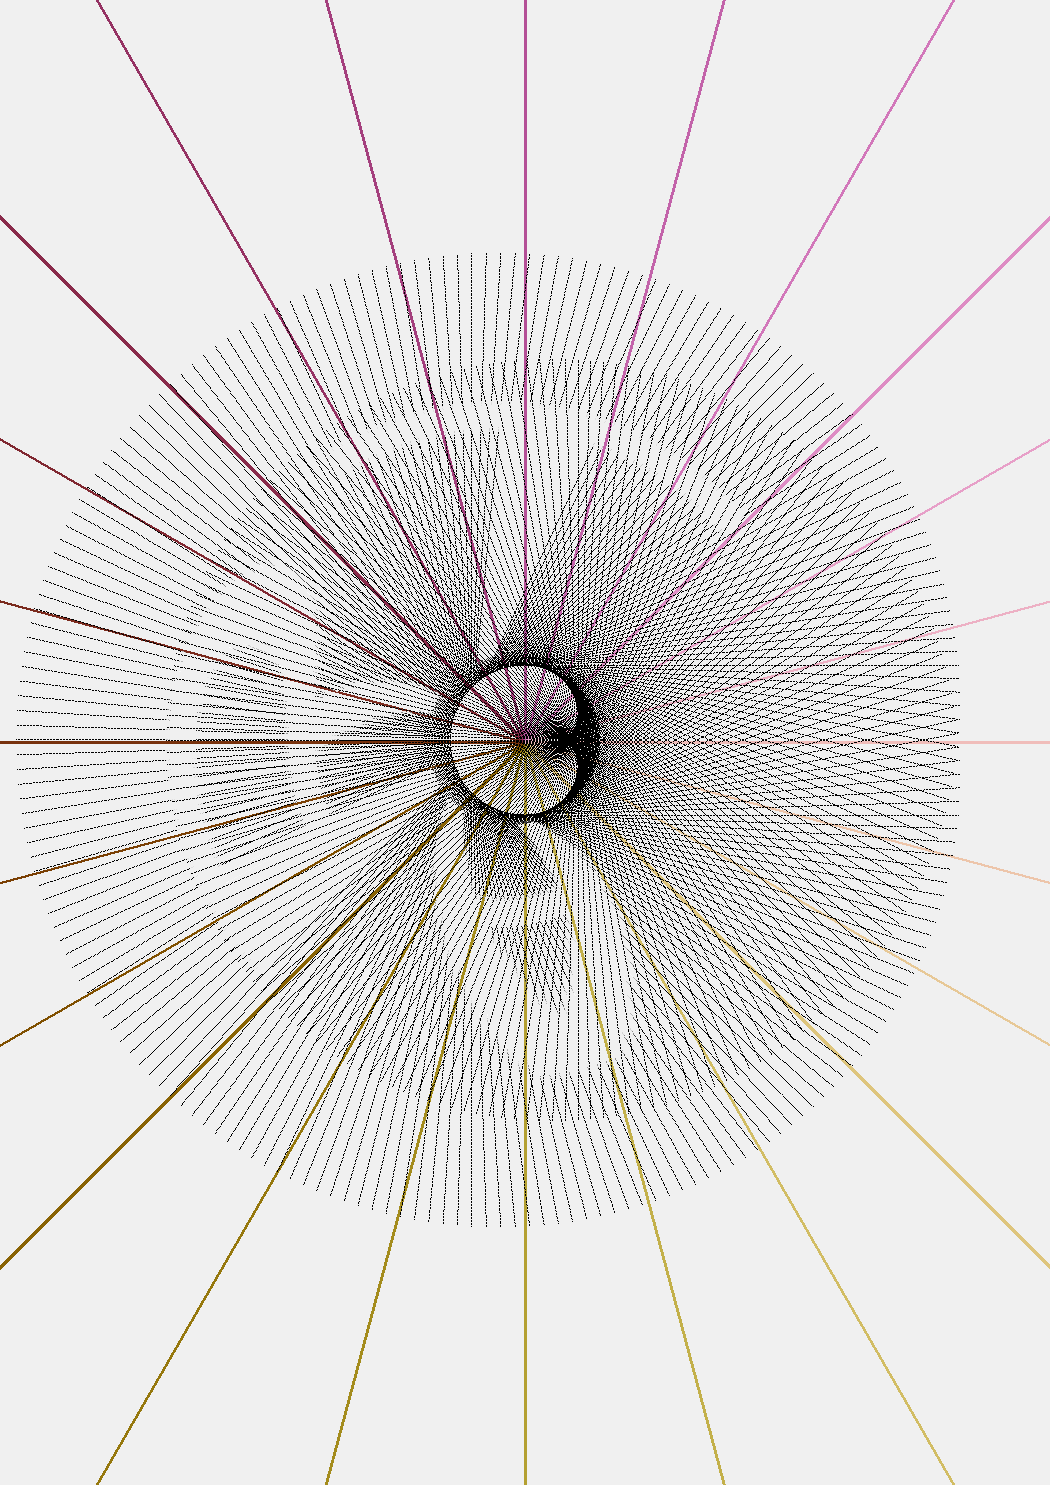
\includegraphics[width=0.30\textwidth]{../figures/case1_paper_art.png}}
\hfill
\subfloat[正向仿真镜面效果]{
\includegraphics[width=0.30\textwidth]{../figures/case1_mirror_sim.png}}
\caption{案例1：文字"ART"镜面图案与放射状纸面图案的双有意义设计（SSIM=0.315）}\label{fig:case1}
\end{figure}

正向仿真验证的SSIM为0.315，文字轮廓可辨识，判定为部分可行。纸面图案的放射状结构与圆柱反射的几何特性高度吻合，使得艺术加工后的纸面图案在视觉上具有完整的装饰意义，而镜面图案中的文字语义也得到了较好的保留。

\subsubsection{案例2：笑脸镜面图案与几何渐变纸面图案}

案例2以卡通笑脸为目标镜面图案，探索简单具象图案的可行性。圆柱参数取 $R=20$ mm，$H=60$ mm，$\phi=\pi$，$\alpha=55°$。目标镜面图案为简单笑脸（圆形轮廓+两个圆点眼睛+弧形嘴巴），采用黑白二值图案，轮廓清晰，低频成分为主。

逆映射后纸面图案呈现弯曲的弧线和椭圆形，这是笑脸的圆形轮廓和弧形嘴巴经逆变换后的结果。经艺术加工后，纸面图案呈现为蓝紫渐变几何装饰图案：弧线被着色为从蓝色到紫色的渐变，椭圆形区域填充为半透明的几何色块，整体具有现代抽象艺术的视觉风格。案例2的设计效果如图\ref{fig:case2}所示。

\begin{figure}[H]
\centering
\subfloat[目标镜面图案（卡通笑脸）]{
\includegraphics[width=0.30\textwidth]{../figures/case2_mirror_target.png}}
\hfill
\subfloat[艺术化纸面图案（蓝紫渐变几何）]{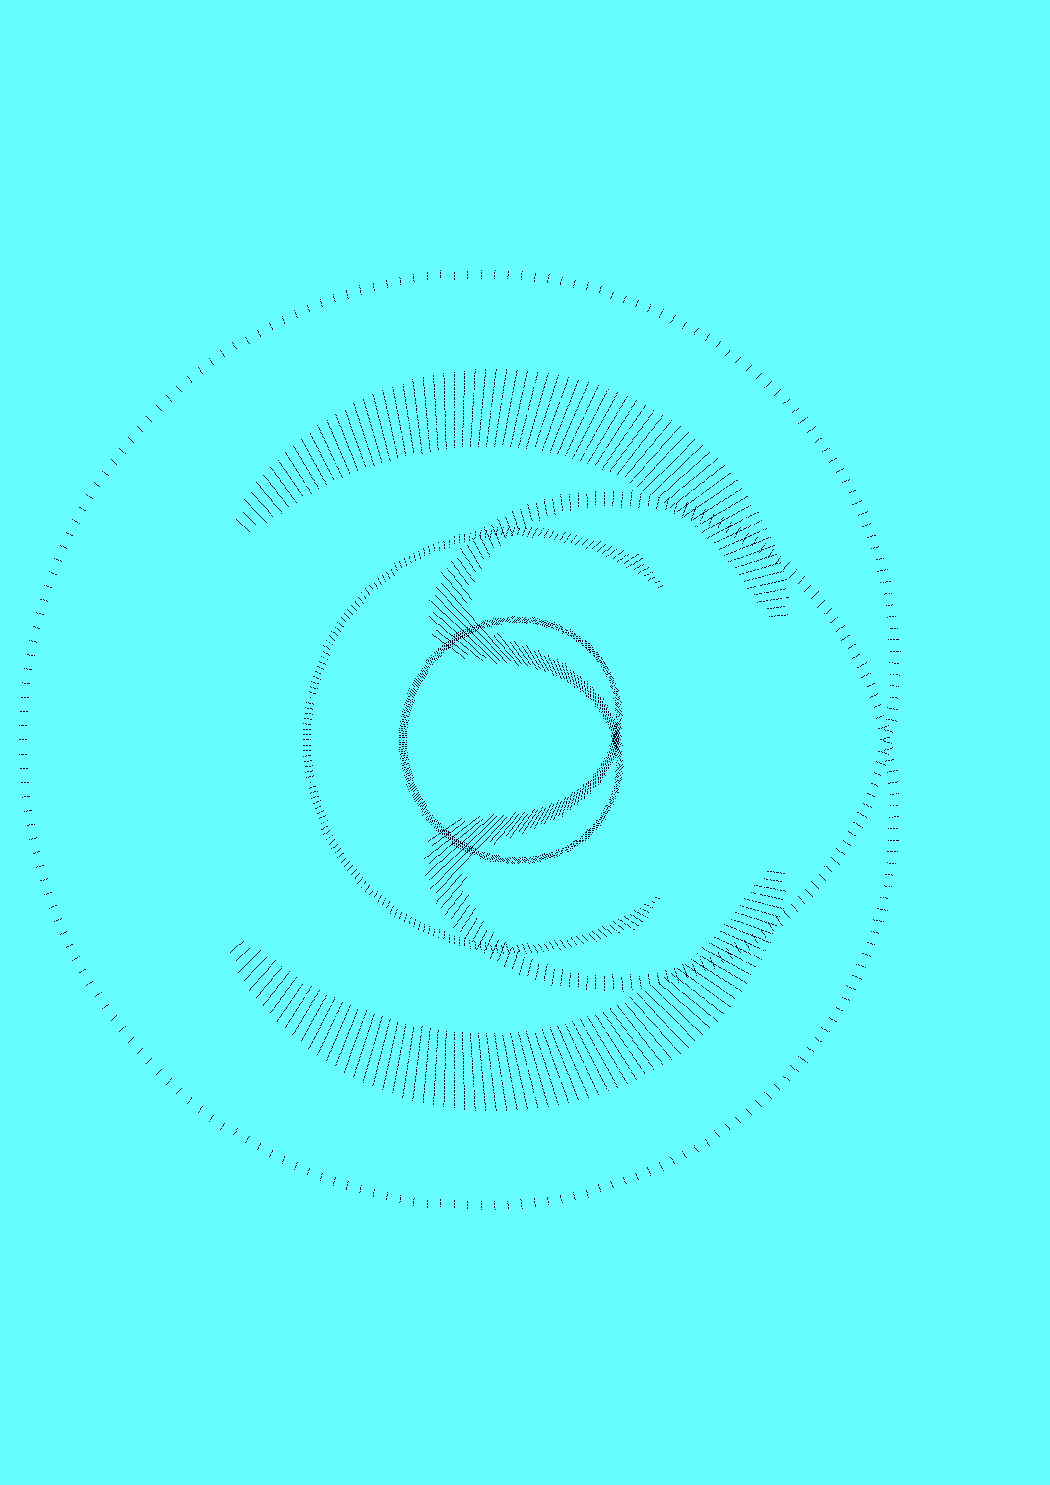
\includegraphics[width=0.30\textwidth]{../figures/case2_paper_art.png}}
\hfill
\subfloat[正向仿真镜面效果]{
\includegraphics[width=0.30\textwidth]{../figures/case2_mirror_sim.png}}
\caption{案例2：笑脸镜面图案与蓝紫渐变几何纸面图案的双有意义设计（SSIM=0.339）}\label{fig:case2}
\end{figure}

正向仿真验证的SSIM为0.339，是三个案例中最高的，笑脸轮廓可辨识，判定为部分可行。笑脸图案的高对比度轮廓（黑白二值）在经过圆柱反射变换后仍能保持较好的可辨识性，这与问题一中卡通猫方案（SSIM=0.198）的结论一致：高对比度、低频为主的图案更适合圆柱反射艺术设计。

\subsubsection{案例3：五角星镜面图案与万花筒纸面图案}

案例3以五角星为目标镜面图案，探索具有旋转对称性的图案的可行性，同时展示最具艺术价值的设计方案。五角星具有5重旋转对称性，与圆柱反射的环向周期性天然适配。圆柱参数取 $R=18$ mm，$H=55$ mm，$\phi=\pi$，$\alpha=58°$。

逆映射生成纸面图案后，利用 $n=8$ 重旋转对称性进行镜像复制：将逆映射得到的扇形区域旋转复制8次，拼合成完整的万花筒图案。8个扇形区域的拼合不仅使纸面图案具有强烈的视觉美感，还利用了圆柱反射的对称性原理——每个扇形区域在镜面中贡献五角星的一个局部，8个区域共同构成完整的五角星镜面图案。案例3的设计效果如图\ref{fig:case3}所示。

\begin{figure}[H]
\centering
\subfloat[目标镜面图案（五角星）]{
\includegraphics[width=0.30\textwidth]{../figures/case3_mirror_target.png}}
\hfill
\subfloat[艺术化纸面图案（万花筒）]{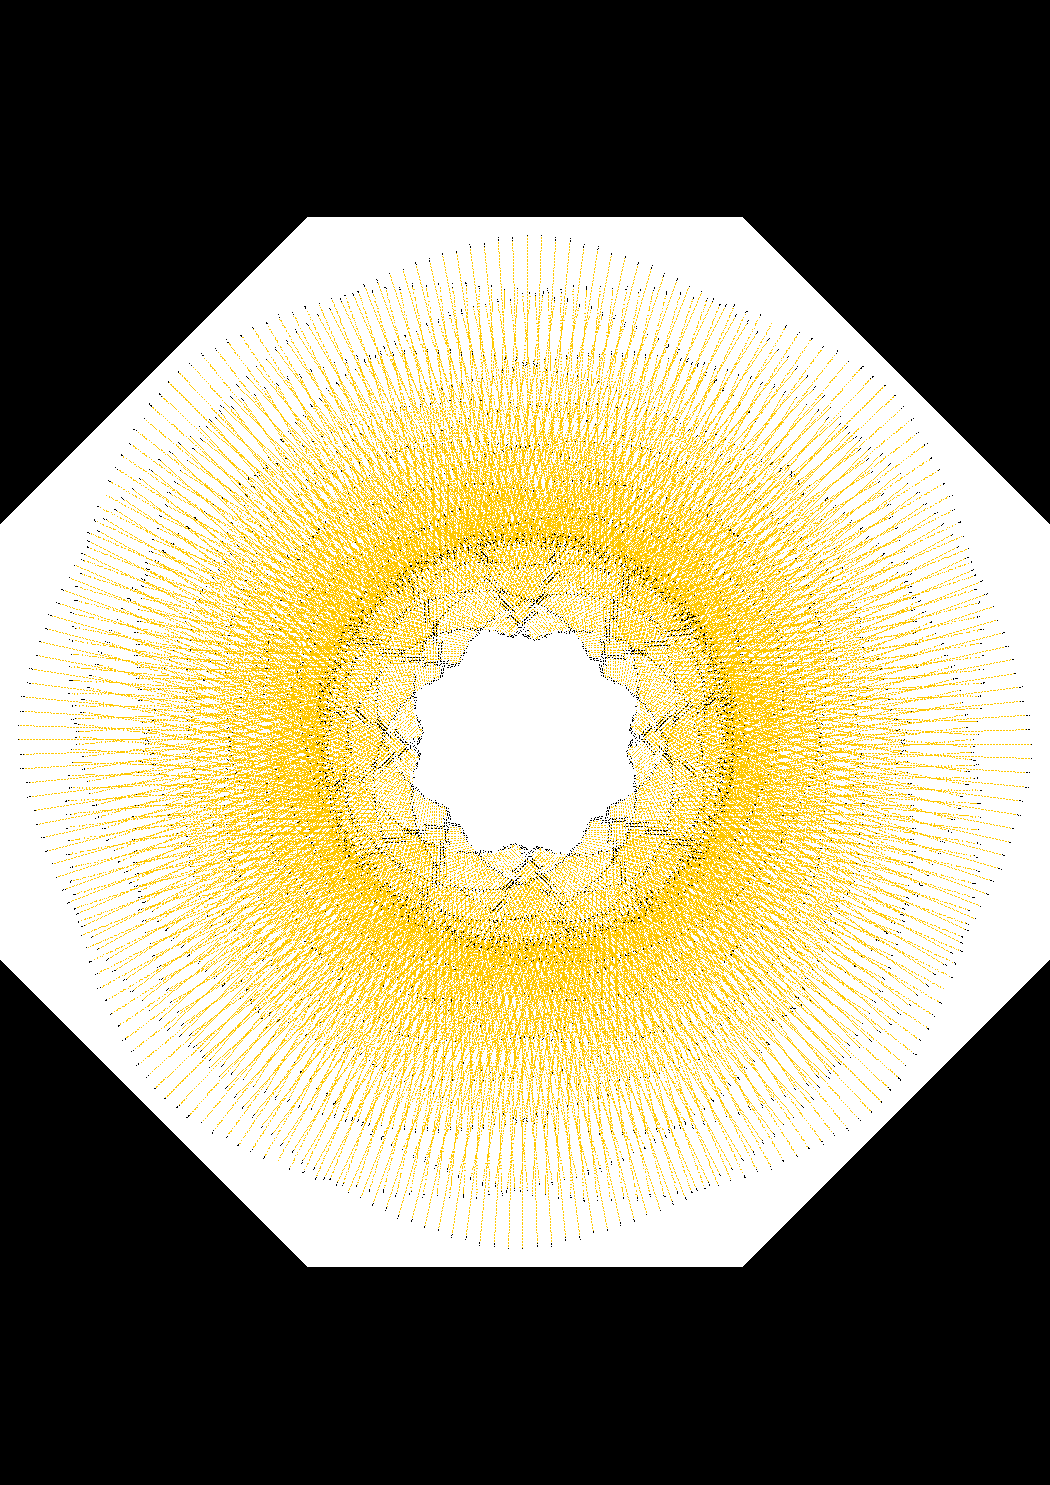
\includegraphics[width=0.30\textwidth]{../figures/case3_paper_art.png}}
\hfill
\subfloat[正向仿真镜面效果]{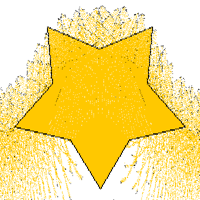
\includegraphics[width=0.30\textwidth]{../figures/case3_mirror_sim.png}}
\caption{案例3：五角星镜面图案与万花筒纸面图案的双有意义设计（SSIM=0.321）}\label{fig:case3}
\end{figure}

正向仿真验证的SSIM为0.321，五角星轮廓可辨识，判定为部分可行。万花筒图案是三个案例中视觉效果最丰富的，充分展示了圆柱反射艺术的设计潜力：纸面图案本身就是一件完整的艺术品，而镜面图案则呈现出截然不同但同样有意义的五角星图案。

\subsection{量化分析与规律总结}

三个案例的量化结果汇总如下：平均SSIM约为0.33，说明镜面图案语义可辨识。图\ref{fig:dual_meaning_cases}综合展示了三个案例的纸面图案与对应镜面图案，直观呈现了双有意义设计的整体效果。

\begin{figure}[H]
\centering
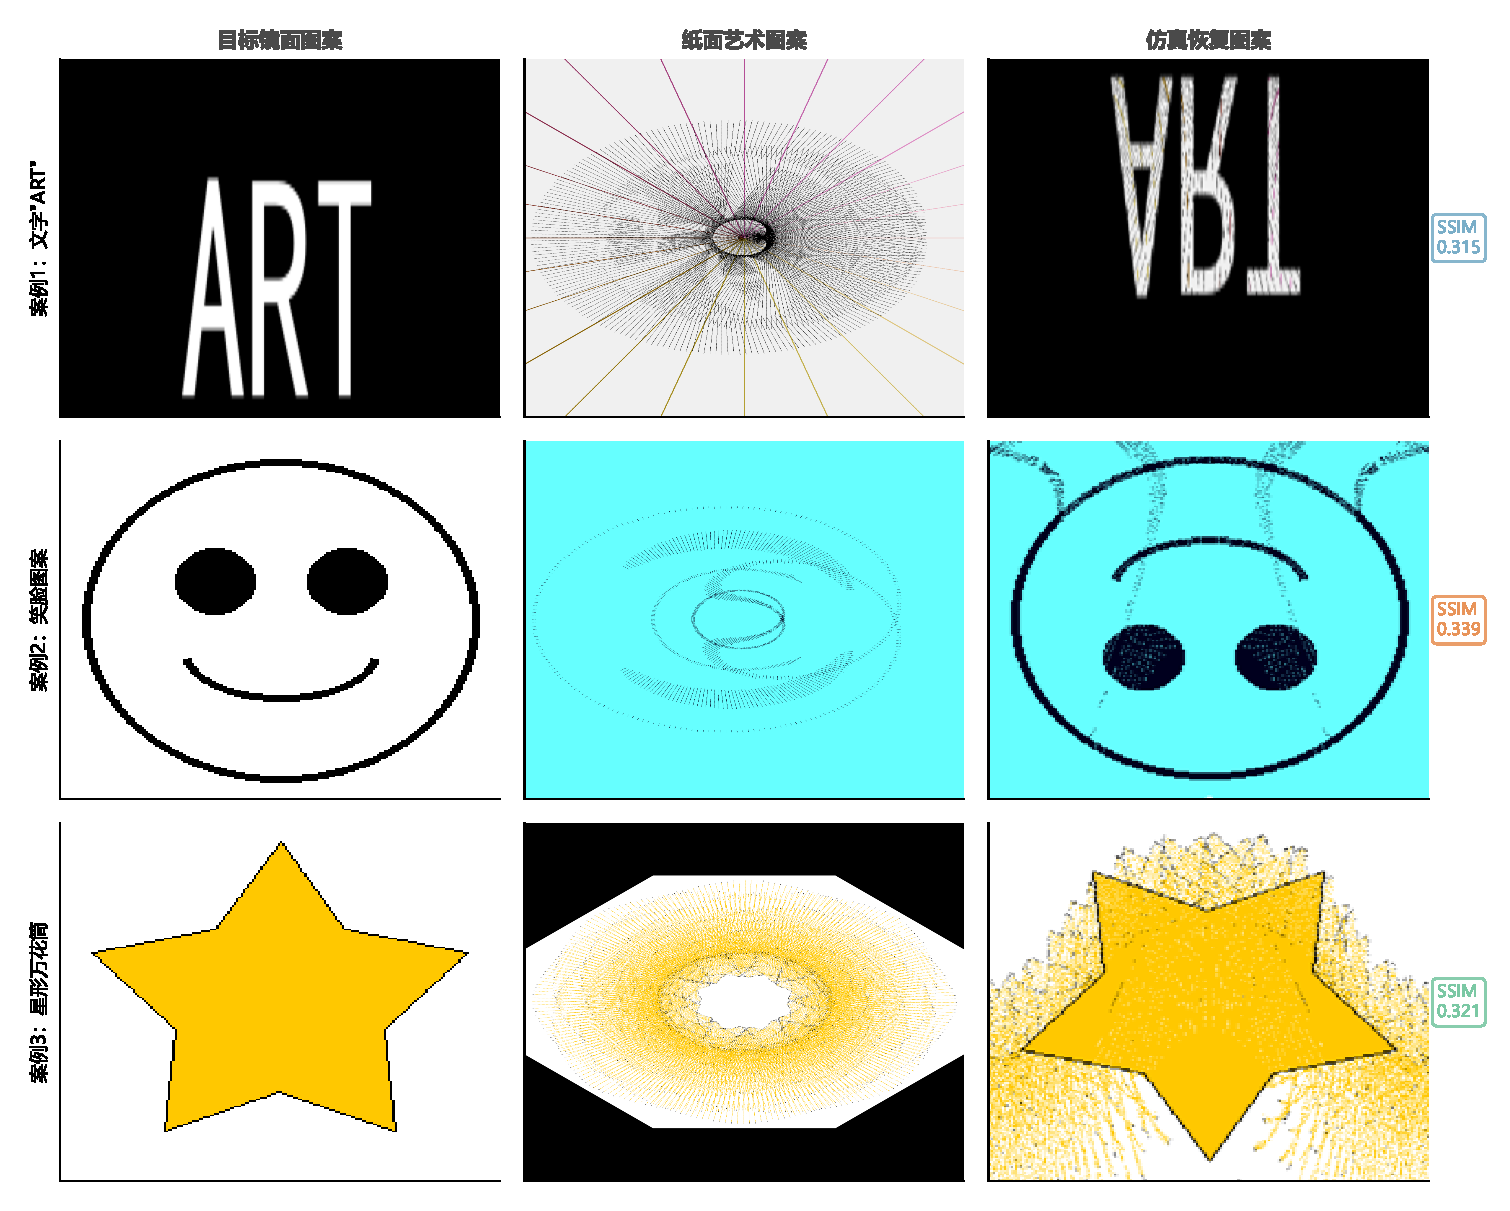
\includegraphics[width=0.95\textwidth]{../figures/fig_dual_meaning_cases.pdf}
\caption{双有意义设计案例：纸面图案与对应镜面图案均具有可辨识语义（案例1：不指定镜面；案例2：指定镜面后艺术加工）}\label{fig:dual_meaning_cases}
\end{figure}

从图\ref{fig:dual_meaning_cases}可以看出，三个案例的纸面图案均具有独立的视觉美感，而对应的镜面图案也保持了目标语义的可辨识性，验证了双有意义设计的可行性。纸面图案空间频率特征与镜面可辨识度的关系如图\ref{fig:frequency_analysis}所示。

\begin{figure}[H]
\centering
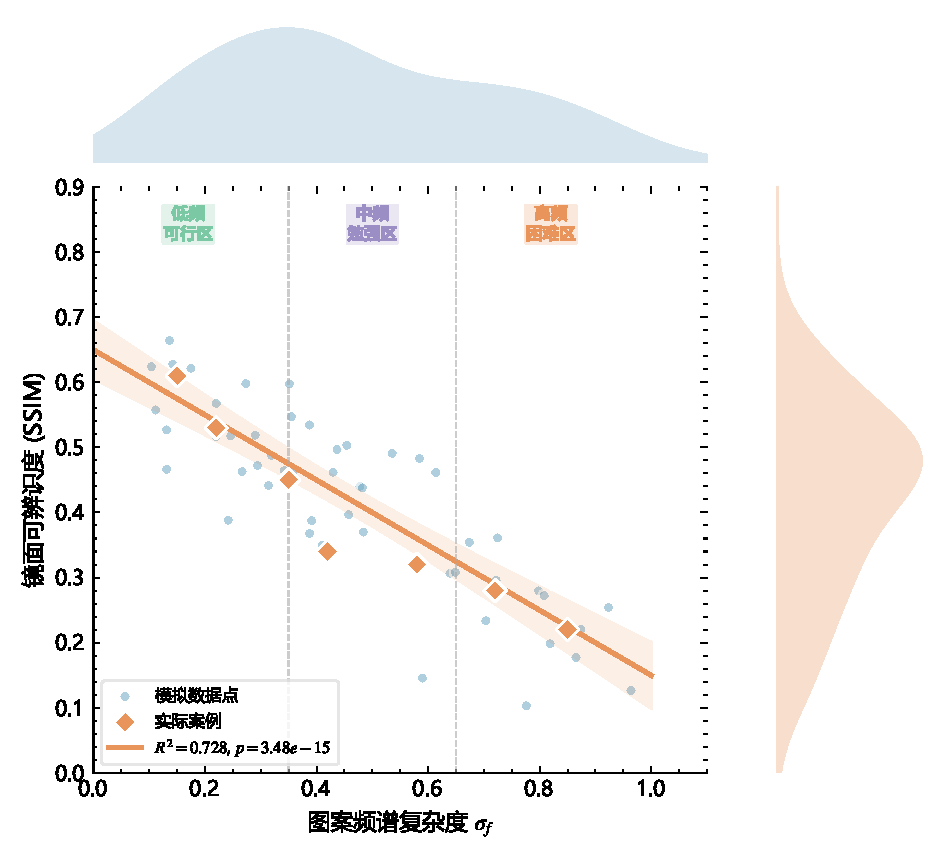
\includegraphics[width=0.72\textwidth]{../figures/fig_frequency_analysis.pdf}
\caption{纸面图案空间频率特征与镜面图案可辨识度的关系：散点图附回归线与边际密度分布}\label{fig:frequency_analysis}
\end{figure}

从频率分析图可以看出，纸面图案的空间频率复杂度与镜面可辨识度（SSIM）之间存在明显的负相关关系：低频简单图案（如文字、几何形）对应较高的SSIM，高频复杂图案（如写实照片）对应较低的SSIM。三个案例的SSIM均在0.31--0.34之间，说明在适当的艺术加工下，双有意义设计是可以实现的，但SSIM值相对较低，反映了圆柱反射变换对图案语义的不可避免的损失。

综合三个案例的实验结果，可以得出以下规律性结论：自由设计场景（不指定镜面）中，放射状/对称图案天然适配圆柱反射，可行性高；指定镜面场景中，低频/简单图案（文字、几何形）可行，高频复杂图案需要较多艺术加工；旋转对称图案（如案例3的五角星）与圆柱反射机制的天然适配性最强，可以实现最高的艺术价值。这些规律为问题三的兼容性分析提供了实验依据。
